The importance of dynamics in proteins is highlighted in intrinsically disordered proteins (IDP).
In contrast with more traditionally studied proteins,
they do not need to adopt a defined three-dimensional fold to achieve their function.
Instead, they remain in a disordered, more coil-like state,
where no particular well-defined conformation is adopted by the protein.
In fact, for many IDP's there function seems to depend on the protein remaining in this disordered state most of the time,
only folding upon interaction
(\cite{van2014}).

Fully structured proteins and IDP's are only two ends of a spectrum, 
with a lot of possibilities in between (Fig. \ref{fig:structure_disorder}).
In fact, many structured proteins have at least some intrinsically disordered regions (IDR's).
For example,
it is estimated that 44 percent of the human proteins contain a disordered region of 30 amino acids or more.
Initially, those regions were thought to be linkers between functional, structured regions, but remaining passive otherwise.
However, it has now been established that these regions participate in a variety of functions,
such as interacting with other domains and post translational modifications (PTM's).
Other functionalities include molecular recognition,
molecular assembly,
and entropic chains
(\cite{van2014}).

~\begin{figure}[h!]
	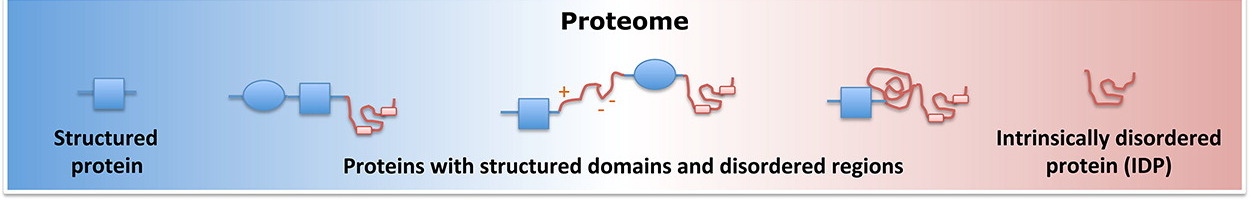
\includegraphics[width=\linewidth]{./literature_review/proteins/dynamics/img/protein_classes.jpeg}
	\caption{
	\textbf{Order and disorder in proteins.}
Proteins exist as a spectrum of dynamical possibilities,
ranging from fully structured and relatively rigid 
to fully disordered.
(adapted from \cite{van2014}).
}
	\label{fig:structure_disorder}
~\end{figure}
